\section{Calc-Regular Languages}
\label{2.0}
\subsection{Overview}
\label{2.1}
Calc-regular languages as presented in the paper by Grosch et al. \cite{Calc-regular-paper} are a formal language class representing length-prefix languages using fixed nesting. The paper lays the groundwork for the research presented in this thesis. The main addition to this new language class was the concept of an 'accumulator'.\\\\ While parsing the contents (usually digits) of the length field of a Calc-regular language, each byte of this length field gets stored inside an accumulator. If the parser recognizes and decides that the end of the length-field has been reached, a function converts the contents of this accumulator into a numerical representation to an arbitrary base. Following this function call, the parser decrements the number now stored in the accumulator by one for every byte of the value field\footnote{The value field contains the actual contents of the message. See \cite{Type-Length-Value}.} read. If the accumulator's value reaches zero, the parser now stops reading value bytes and decides that the end of this specific encoded message has been reached. Now follows either an end-of-content symbol which is distinctly defined by the format used (\em e.g. \em  netstrings) or the first byte of the next message if the format does not use end-of-content symbols (\em e.g. \em protobufs)\footnote{The communication stream could also end instead of another message appearing.}. 
\subsection{Calc-FSM and Calc-Regular Expressions}
\label{2.2}
When talking about formal language classes, establishing some definition of a formal automaton has to be considered. In the case of Calc-regular languages, the Calc-finite state machine (Calc-FSM) was introduced \cite{Calc-regular-paper}. This finite automaton is able to deterministically handle Calc-regular language inputs of any kind. The Calc-FSM uses an accumulator the way it has been described in \hyperref[2.1]{the chapter prior to this.} \hyperref[fig:Calc-FSM]{Figure 1} describes the core functionality of a Calc-FSM. The keyword \texttt{'store'} refers to the accumulator storing the digit read, \texttt{'-1'} refers to the accumulator decrementing its value by one, and \texttt{'=0'} represents the condition that the accumulator's value is equal to zero. What is missing in this representation of the Calc-FSM is the function which converts the stored digits into a numerical representation of the number read. In this example for netstrings, this function gets called during the transition from \textbf{state 1} to \textbf{state 2}.
\begin{figure}
    \centering
    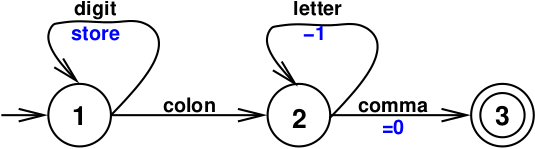
\includegraphics[width=0.6\linewidth]{fig/Calc-fsm-example-2.png}
    \caption{Basic functionality of a Calc-FSM for netstrings.}
    \label{fig:Calc-FSM}
\end{figure}\\\\
It is also important to mention that Grosch et al. established Calc-regular expressions based on the concept of regular expressions. For a much more in-depth explanation on Calc-regular languages and therefore the foundations of this thesis' work, we recommend reading the author's findings in their respective publication \cite{Calc-regular-paper}.
\subsection{Limitations of Calc-Regular Languages}
\label{2.3}
As already described above, Calc-regular languages define length-prefix languages with \textit{fixed} nesting.
This solid theoretical foundation describes the underlying problem really well but when looking at practical examples of length-prefix formats we can see its limitations. Most of the frequently used formats (\textit{e.g.} protobuf \cite{google-protobuf-encoding}, ASN.1 \cite{ASN.1}) employ \textit{variable} nesting and can therefore not be characterized by using Calc-regular languages. The distinction between \textit{fixed} and \textit{variable} nesting shall not be underestimated, as a formal definition for this type of languages is much more complex than it may sound at first. In this thesis we will present an extension to the aforementioned Calc-regular languages which shall ultimately be able to handle length-prefix languages using variable nesting.
In Grosch et al.'s paper \cite{Calc-regular-paper} they acknowledge the possibility for this extension and refer to it as 'Calc-context-free languages'. During our research, however, we have decided to name this extended language class 'Calc-LL(1)' instead.
